% id: 31-24
% book: 개념원리 중학 3-2 · 03 임의의 예각의 삼각비의 값
% section: 중단원 마무리하기 STEP 3 실력 UP
% figure: crop:fig-31-24.png
% answer: $\dfrac{\sqrt{6}-\sqrt{2}}{4}$
% answer_source: 답지(쪽 렌더)
% variant_level: 0 (원본 전사)
% 이 파일은 build.mjs 가 items.json 에서 만든다. 고칠 때는 items.json 을 고친다.
\smash{\raisebox{1.5mm}{\dmkichul{개념원리 중학 3-2 31쪽 24번}}}
\noindent\begin{minipage}[t]{0.58\linewidth}\vspace{0pt}\raggedright 오른쪽 그림과 같은 직사각형~$\pt{ABCD}$에서 $\seg{AB}=3$이고 $\angle\pt{AEF}=90^\circ$, $\angle\pt{BAE}=30^\circ$, $\angle\pt{EAF}=45^\circ$일 때, $\sin 15^\circ$의 값을 구하시오.\end{minipage}\hfill\begin{minipage}[t]{0.4\linewidth}\vspace{0pt}\centering \setlength{\dmfigw}{88.0pt}\ifdim\dmfigw>\linewidth\setlength{\dmfigw}{\linewidth}\fi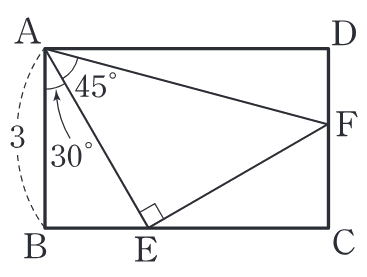
\includegraphics[width=\dmfigw]{figures/fig-31-24.png}\end{minipage}\par
